%Estado del arte y arquitectura propuesta
Previo al diseño del sistema de adquisición de datos para detectores de muones, es pertinente conocer el estado del arte de otros sistemas de adquisición para física de partículas, con el fin de contrastar y rescatar las diferentes estrategias y tecnologías empleadas en la actualidad.

Como referencia para el diseño del sistema de adquisición, se han investigado detectores como los descritos en \cite{Basiladze2017Methods1} y \cite{Basiladze2017Methods2}, enfocados a detección de partículas en diferentes rubros y condiciones. En este capítulo se describen tres sistemas relacionados a esta temática, destacando ideas sobre el esquema general de adquisición de datos, tecnologías que se utilizan actualmente para construirlos y métodos para adquirir y procesar las señales captadas.

\section{LabPet II}
\label{par:labpet}
	Uno de los detectores estudiados es LabPet II \cite{Njejimana2013DesignImaging}, detector que posee un DAQ (Data Acquisition system) distribuido en tres etapas donde cada una de ellas está compuesta por una FPGA, tal como se ilustra en la Figura \ref{fig:njejimana}. Una primera etapa llamada \textit{Front-End board} se encarga de registrar tiempo, energía y posición de las partículas captadas; una segunda etapa llamada \textit{Hub board} ordena cronológicamente los eventos capturados, mientras que una tercera etapa llamada \textit{Coincidence board} agrupa detecciones coincidentes, calculando además la tasa de eventos aleatorios ocurridos. Esta última etapa es capaz de recibir datos desde múltiples Hub boards para luego enviarlos a un computador.
	
	%La Figura \ref{fig:njejimana} ilustra LabPet II \gcnote{dangling modifier. Estas cometiendo los mismos errores que antes.}. Se \gcnote{otro mas} compone de 3 FPGAs: una encargada de capturar las señales provenientes de los detectores, llamada \textit{Front-End board}; otra dedicada a ordenar los eventos y corregir datos, llamada \textit{Hub board}; y una última FPGA encargada de seleccionar eventos válidos y coincidentes, llamada \textit{Coincidence board}, la cual puede conectarse a múltiples Hub boards. \gcnote{Suena redundante con el parrafo anterior. Juntar y uniformar ambos parrafos.} Los resultados son enviados a un computador, el cual también permite configurar y ajustar parámetros en las Hub y Coincidence boards.
	
	Si bien los detectores de LabPet II están diseñados para otro tipo de partículas (positrones), la naturaleza de las señales es muy similar a los muones, y por lo tanto la lógica para su adquisición y procesamiento es comparable. Aún así, la cantidad de señales que es capaz de manejar dicho dispositivo ronda las 64 señales por módulo, a tasas cercanas a los 2 millones de eventos por segundo, las que comparativamente sobrepasarían las necesidades del sistema a desarrollar en este proyecto de titulación. Por ejemplo, los rayos muones cruzan la corteza terrestre a aproximadamente 1 muon por minuto en un área de 1 cm$^2$\cite{Rocca2018CosmicUs}, muy por debajo de lo que se espera en LabPET II. Replicar un sistema como LabPet II para sTGC minería sería factible, pero implicaría un uso de recursos mayor al realmente necesario, ya que se podrían alcanzar los objetivos propuestos para sTGC minería con un sistema de menor tamaño, por ejemplo utilizando solo una FPGA por módulo de detección en vez de dos o tres.
	
	Del sistema de adquisición para LabPet II se destaca la utilización de multiplexores, serializadores/deserializadores y memorias de almacenamiento temporal (\textit{buffer}). Dada la naturaleza y cantidad de eventos, se hace necesario serializar la información, ya que de otro modo sería necesario construir dispositivos con múltiples puertos de entrada o incluir varios del mismo tipo. Además, debido a la frecuencia de los eventos, se hace obligatoria la existencia de \textit{buffers} para el almacenamiento de la información, permitiendo procesarlos y transmitirlos hacia etapas posteriores a tasas menores. Es destacable también la utilización de métodos para ordenar cronológicamente los eventos y la implementación del método TOT (Time-over-threshold)\cite{Orita2018TheSystem} para el cálculo de energía y datos temporales de pulsos analógicos. Este último es el método utilizado por la interfaz de lectura presente en el proyecto sTGC Minería.
	
	\begin{figure}[h]
		\centering
		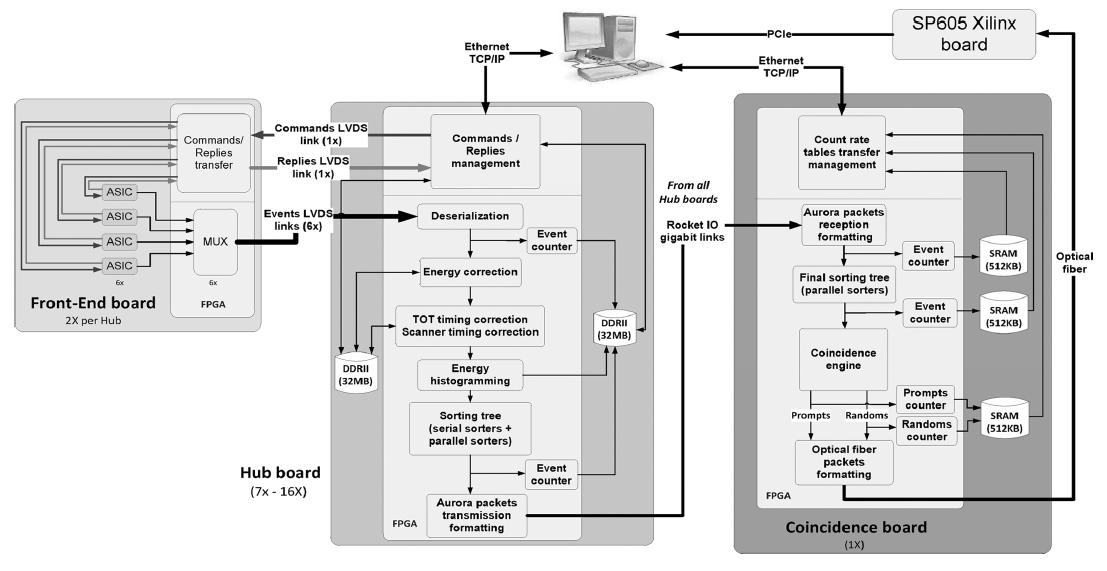
\includegraphics[scale=0.45]{njejimana.png}
		\caption{Diagrama de bloques del sistema de adquisición de datos para LabPET II \cite{Njejimana2013DesignImaging}}
		\label{fig:njejimana}
	\end{figure}
	
\newpage
\section{4D PET}
\label{par:4dpet}
	Otro sistema de referencia es el DAQ para el sistema modular 4D PET \cite{Marcatili2011DevelopmentDetector}. Este dispositivo permite capturar entre 144 a 576 señales provenientes de arreglos matriciales de fotomultiplicadores. Se caracteriza principalmente por poseer una tarjeta madre central, en la cual es posible conectar hasta 18 tarjetas de adquisición. Cada una de estas tarjetas tiene de 8 a 32 canales para adquisición de señales, y su función es capturar, procesar y enviar información a la placa madre. La Figura \ref{fig:marcatili} ilustra la arquitectura de este sistema.
		
	Las señales son capturadas por ASICs (\textit{Application Specific Integrated Circuits}), muestreadas por conversores análogo-digitales y procesadas por una FPGA, mientras que una FPGA principal (etiquetada como Master FPGA) se encarga de controlar a las FPGAs anteriores y de recibir los datos capturados. El procesamiento inicial de las señales se encarga de calcular energía y datos temporales asociados a las partículas detectadas, mientras que el procesamiento final relaciona los eventos que hayan sido temporalmente coincidentes entre sí y a su vez calcula el tiempo de vuelvo de las partículas, mediante un conversor de tiempo a señal digital (TDC).
	       	
	Este sistema destaca por su modularidad, la cual permite un fácil escalamiento. En contraste con LabPET II, se utilizan varias placas adquisidoras paralelas en vez de utilizar serialización de datos, permitiendo procesar la información antes de llegar a la FPGA principal. Cabe destacar que esta arquitectura está relacionada con la necesidad de encontrar múltiples eventos simultáneos en distintas ubicaciones, requerimiento que no está presente en el sistema que se planea diseñar para este proyecto de titulación. 
	
	\begin{figure}[h]
		\centering
		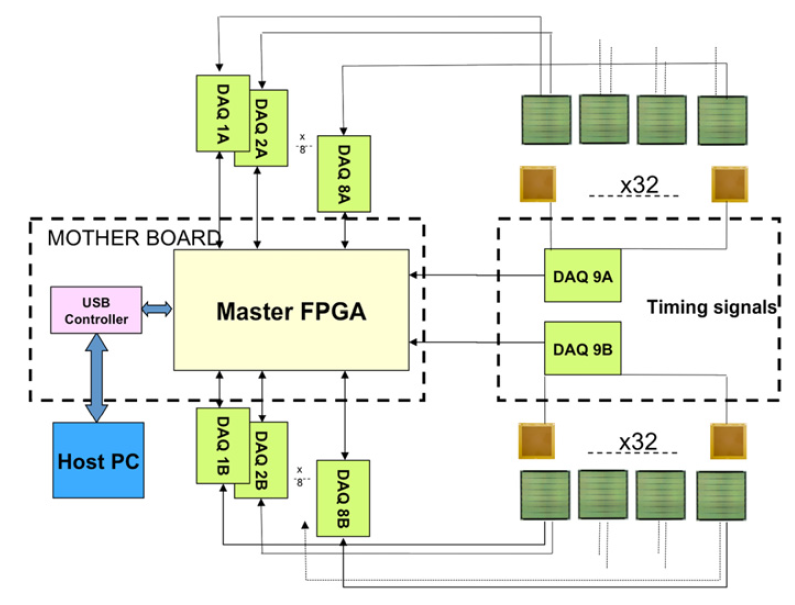
\includegraphics[scale=0.4]{marcatili.png}
		\caption{Diagrama de bloques del sistema de adquisición de datos para Detector PET 4D \cite{Marcatili2011DevelopmentDetector}}
		\label{fig:marcatili}
	\end{figure}
	
\newpage
\section{ATLAS}
\label{sec:atlas}
	Finalmente, la referencia más importante corresponde al experimento ATLAS \cite{Spieler2012ElectronicsAcquisition}, ya que una de sus etapas utiliza detectores sTGC, mientras que otra de sus etapas utiliza la misma interfaz de lectura que será utilizada en sTGC Minería.

	El experimento ATLAS se encarga de interceptar grupos de partículas provenientes de haces de protones acelerados en el LHC (Large Hadron Collider) en CERN, con el objetivo de estudiar las colisiones de partículas ocurridas a su paso. Las colisiones se generan aproximadamente cada 25$\mu$s\cite{Whiteson2016TheSystem}, y cada colisión produce cerca de 23 interacciones con el detector, que junto a otros factores implica cerca de 10$^9$ eventos cada segundo. La tasa de aparición y nivel de energía de estos eventos son las principales razones por las que este detector es tecnológicamente complejo.
	
	El estudio de colisiones tiene como objetivo medir partículas conocidas y deducir la existencia de partículas nuevas. Para lograrlo, es necesario reconstruir las trayectorias e interacciones de todas las partículas medibles mediante múltiples y variados sistemas de detección. Uno de estos sistemas corresponde al Espectrómetro de Muones\cite{Pontecorvo2004TheSpectrometer}, el cual permite determinar la validez de los eventos y trazar la trayectoria de los muones emitidos en las colisiones. 
	
	El Espectrómetro de Muones se compone de múltiples tecnologías de detección diferentes, una de las cuales corresponde a los detectores sTGC ubicados en la Small Wheel, mencionada en la Sección \ref{par:smallwheel}. Otra de las tecnologías de detección que componen al Espectrómetro corresponde a los detectores TGC (Thin Gap Chamber), los cuales se diferencian de los detectores sTGC en el tamaño de sus componentes. Los detectores TGC están ubicados en el sector denominado Big Wheel, indicado en la Figura \ref{fig:both-wheels}, y sus datos son obtenidos gracias a una interfaz de lectura llamada ASD (Amplificator-Shaper-Discriminator). Esta interfaz de lectura, en conjunto con detectores sTGC, da vida al proyecto sTGC Minería en CCTVal, y su funcionamiento será explicado con mayor detalle en el Capítulo \ref{cap:sdet}.
	
	\begin{figure}[h]
		\centering
		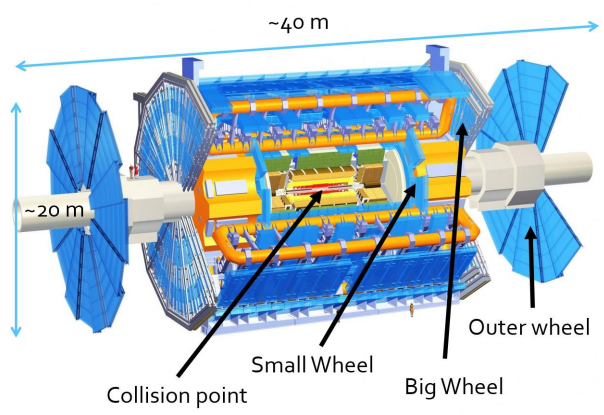
\includegraphics[scale=0.5]{atlas-layout-big-small-wheel.png} 
		\caption{Layout del experimento ATLAS, donde se indica la posiciónde la Small Wheel y la Big Wheel\cite{Formenti2018CERNReport}}
		\label{fig:both-wheels}
	\end{figure}
	
	La Figura \ref{fig:spieler} ilustra el sistema de captura de datos para detectores TGC del Big Wheel en el Espectrómetro de Muones. Los muones son representados con el símbolo $\mu$ y cruzan tres capas de detectores TGC, cada una de las cuales cuenta con sus interfaces de lectura ASD. Los bloques posteriores se encargan de pre-procesar los pulsos capturados y entregarlos a las posteriores etapas de lectura y de selección de eventos.
	
	\begin{figure}[h]
		\centering
		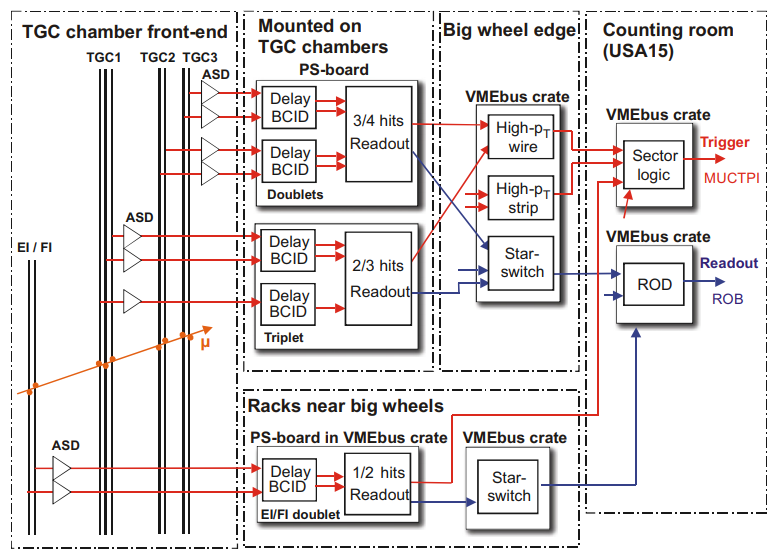
\includegraphics[scale=0.6]{spieler.png}
		\caption{Diagrama de la interfaz de captura para detectores de muones TGC \cite{Spieler2012ElectronicsAcquisition}. Los muones se representan con el símbolo $\mu$. Existen 3 capas de detectores, por lo tanto se observan 3 bloques que incluyen retardos, selección y captura de los pulsos.}
		\label{fig:spieler}
	\end{figure}

	En ATLAS, la selección de eventos a ser estudiados se lleva a cabo en dos etapas. La primera de ellas, llamada \textit{Level 1 Trigger}, involucra al Espectrómetro de Muones y calorímetros. La segunda etapa involucra algoritmos distribuidos en varios computadores y se le conoce como \textit{High-level Trigger}. La Figura \ref{fig:colombo} ilustra ambas etapas en paralelo a los sistemas de lectura de datos. El sistema de lectura de datos ilustrado en \ref{fig:spieler} corresponde al cuadro amarillo ubicado en la esquina superior derecha de la Figura \ref{fig:colombo}, etiquetado como \textit{Muon}. Si el Level 1 Trigger aprueba un evento detectado por el Espectrómetro y los calorímetros, entonces inicia la adquisición de estos datos en la tarjeta de lectura (etiquetada como \textit{Readout System} en la Figura \ref{fig:colombo}). Además, el Level 1 Trigger envía información sobre regiones de interés a analizar, con el fin de llevar a cabo la segunda etapa de selección (\textit{High-Level Trigger}). Esta segunda etapa de selección utiliza software distribuido en cerca de 2000 computadores conectados a una red Ethernet y filtra eventos en función a muestras de datos pertenecientes a las regiones de interés calculadas por el Level 1 Trigger\cite{Colombo2015Data-flowCase}. Finalmente, los eventos seleccionados son trasferidos y  almacenados en los bancos de datos del centro de investigación.
	
	\begin{figure}[h]
		\centering
		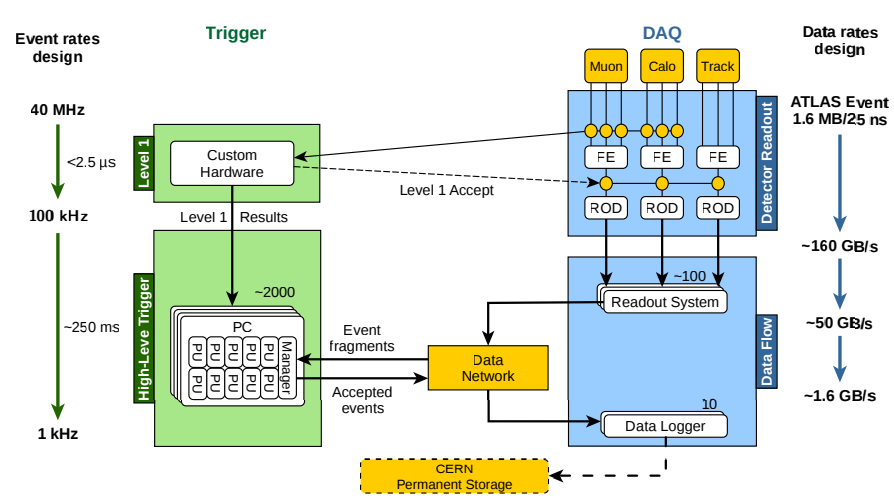
\includegraphics[scale=0.56]{colombo.png}
		\caption{Diagrama del sistema de disparo y adquisición de datos en el experimento ATLAS. \cite{Colombo2015Data-flowCase}}
		\label{fig:colombo}
	\end{figure}
	
	Entrando aún más en detalle respecto a la Figura \ref{fig:colombo}, el verdadero sistema de adquisición de datos en ATLAS es un software distribuido en red\cite{Whiteson2016TheSystem}, capaz de discriminar, procesar y transferir los eventos seleccionados hacia los bancos de almacenamiento de datos. El sistema de lectura (\textit{Readout System}), en conjunto con el Level 1 Trigger, solo sería un equivalente a una interfaz de captura muy sofisticada. Para el caso de esta memoria de titulación, el Readout System del experimento ATLAS sería comparable, en términos de sus niveles de complejidad y de los bloques lógicos que los componen, al sistema de adquisición de datos que se desea diseñar para sTGC Minería.
	
	El Readout System de ATLAS consiste en una tarjeta llamada ROBIN, compuesta de buffers, chips de comunicación, memoria flash, un procesador y una FPGA, como se ilustra en la Figura \ref{fig:whiteson}
	
	\begin{figure}[h]
		\centering
		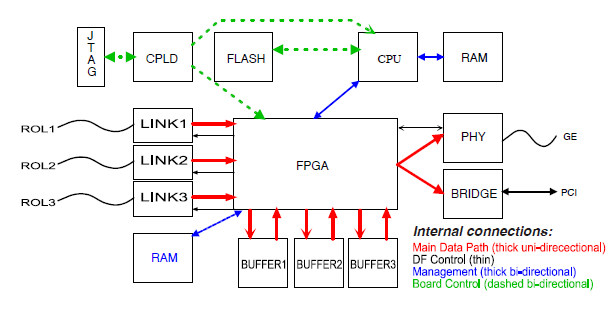
\includegraphics[scale=0.7]{whiteson.png}
		\caption{Diagrama de la tarjeta de lectura ROBIN en ATLAS \cite{Whiteson2016TheSystem}.}
		\label{fig:whiteson}
	\end{figure}
	
	La lógica implementada en la FPGA se ilustra en la Figura \ref{fig:whiteson2}. Se observa que su labor es principalmente controlar los buffers de datos, traspasar los eventos captados hacia la siguiente etapa y eliminar los datos descartados por la señal de disparo de alto nivel.
	
	\begin{figure}[h]
		\centering
		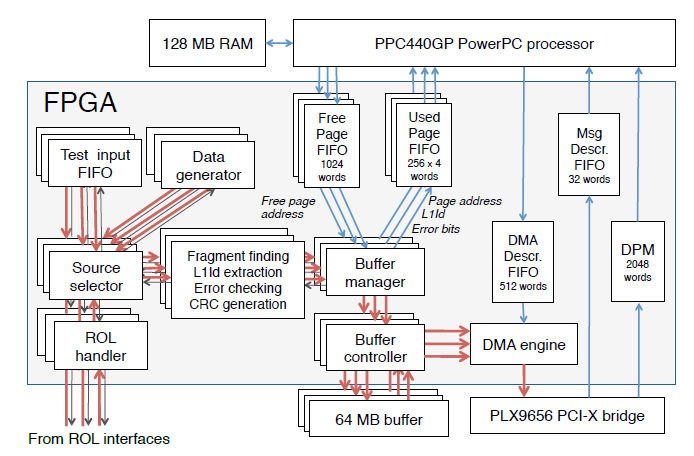
\includegraphics[scale=0.7]{whiteson2.png}
		\caption{Diagrama de bloques de la FPGA en ROBIN \cite{Whiteson2016TheSystem}.}
		\label{fig:whiteson2}
	\end{figure}
	
	\newpage
	Si bien ATLAS es un proyecto con detectores comparativamente más complejos que los descritos en las Secciones \ref{par:labpet} y \ref{par:4dpet}, ATLAS presenta elementos comunes con ellos es su composición, sobretodo en cuanto a la utilización de ASICs y FPGAs para captura y control de los datos adquiridos. ATLAS se asemeja funcionalmente al 4D PET, en el sentido de implementar múltiples instancias de hardware equivalente, para así lograr manejar mayor cantidad de datos y brindar mayor control en cada uno de ellos. El fuerte de ATLAS radica en su conectividad en red y sistemas distribuidos, necesarios para la gran cantidad de datos simultáneos que deben ser procesados.


\section{Discusión sobre alternativas existentes}
	Es claro que la tendencia en desarrollo de sistemas de adquisición es la utilización de ASICs en etapas de primera lectura, mientras que se utilizan FPGAs en etapas de manejo de datos y preprocesamiento, principalmente debido a la magnitud temporal de las señales, a la alta necesidad de precisión en su sincronización, y a la gran cantidad de señales de entrada que deben ser atendidas.
	
	Los elementos más utilizados y recomendados a implementar son los buffers de almacenamiento, principalmente para ajustar la tasa de transmisión de datos de la captura hacia las siguientes etapas de procesamiento, que suelen ser más lentas. En el sistema que se planea diseñar esto no es un problema, ya que la tasa de eventos es muy baja en comparación a los detectores estudiados. Aún así, los buffers pueden ser útiles para el escalamiento de los detectores en el futuro.
	
	El concepto de serialización de datos estuvo principalmente presente en el detector LabPET II. Es pertinente considerarlo, sobretodo para el escalamiento del detector de muones. En caso de requerir cubrir un área mayor o con varias capas superpuestas de detectores, será necesario captar mayor cantidad de señales. Es allí donde se debe decidir si es recomendable comenzar con serialización de datos o con paralelismo de hardware.% Además, dado que es necesario tener noción del tiempo de ocurrencia de los eventos, podría asociarse este dato a cada pulso, facilitando la implementación de serialización de datos. Esto no sería una desventaja, ya que no existe real necesidad de procesar datos de manera rápida y simultanea, reduciendo costos en hardware, pero aumentando esfuerzos de ingeniería.
	
	%Para el caso de pre-procesamiento, selección, formateo y transmisión de datos se puede considerar agregar procesadores dedicados en conjunto con la FPGA principal, que si bien no fueron encontrados textualmente en los ejemplos indicados, sí pueden ser de utilidad, sobretodo dada la existencias de chips que incluyen FPGA en conjunto con procesadores, como los SoC (\textit{System on Chip}) Zynq.
	
	% Finalmente, puede ser interesante incluir métodos de TDC para conversión de la señal digital generada por la placa acondicionadora ASD. La duración de esta señal tiene relación con la amplitud y la energía de los pulsos analógicos captados, lo que podría ser muestreado con una implementación similar a la indicada en \cite{Arpin2010AResources}.
	
	En resumen, es conveniente diseñar el sistema en una FPGA dedicada a la adquisición de datos, incluyendo buffers de almacenamiento para los eventos capturados y replicando este sistema para cada detector adicional.
	